% This is LLNCS.DEM the demonstration file of
% the LaTeX macro package from Springer-Verlag
% for Lecture Notes in Computer Science,
% version 2.4 for LaTeX2e as of 16. April 2010
%
\documentclass{llncs}
%
\usepackage[portuguese]{babel}
\usepackage[utf8]{inputenc}
\usepackage{makeidx}  % allows for indexgeneration
\usepackage{graphicx}
\usepackage{listings}


%

\begin{document}


%
\frontmatter          % for the preliminaries
%
\pagestyle{headings}  % switches on printing of running heads
%
\title{Ano Escolar}
\subtitle{Resolução de Problemas de Otimização utilizando\\
Programação em Lógica com Restrições}
%
\titlerunning{Ano Escolar}  % abbreviated title (for running head)
%                                     also used for the TOC unless
%                                     \toctitle is used
%
\author{João Barbosa \and José Martins}
%
\authorrunning{João Barbosa \and José Martins} % abbreviated author list (for running head)
%
\institute{Faculdade de Engenharia da Universidade do Porto\\
Rua Roberto Frias, sn, 4200-465 Porto, Portugal}

\maketitle              % typeset the title of the contribution

\begin{abstract} %

Para este trabalho foi proposta a resolução de um problema de otimização referente a calendarização de testes e trabalhos de casa numa escola, utilizando programação em lógica com restrições em \textbf{SICStus Prolog}, permitindo variar o numero de turmas, disciplinas, trabalhos de casa por dia e por disciplina, assim como os horários de cada turma.
Foi implementado um conjunto de predicados de modo a aplicar todas as restrições pertinentes para uma boa resolução do problema em questão.

\keywords{computational efficiency, logic programming, Prolog, restraints}
\end{abstract}
%
\section{Introdução}
%
Este projeto esta a ser realizado no âmbito da unidade curricular Programação em Lógica do Mestrado Integrado em Engenharia Informática e Computação, da Faculdade de Engenharia da Universidade do Porto (FEUP).\par
O objetivo do projeto prende-se com a resolução de um problema de otimização, utilizando programação em lógica com restrições.\par
O problema consiste na calendarização de testes e trabalhos de casa de um periodo letivo, com vários parametros váriaveis como o número de turmas, disciplinas, trabalhos de casa (por dia e por disciplina), assim como a existência de diferentes horários para cada turma. Existem também diversas restrições que devem ser respeitadas.\par
Ao longo deste artigo será descrito o respetivo problema com um nivel de detalhe mais elevado, a abordagem levada a cabo pelo grupo para a implementação de uma possivel solução, e as conclusões retiradas acerca da solução implementada.

\newpage
\section{Descrição do Problema}
%

O Problema ''Ano Escolar'' é referente à marcação de testes e TPCs, ao longo do período, sendo que as seguintes restrições devem ser tidas em conta na resolução apresentada:

	\begin{itemize}
	\item Cada disciplina tem 2 testes por período de aulas, que decorrem num conjunto de semanas específico (mais ou menos a meio e no fim do período). 	
	\item Os alunos não podem ter mais do que 2 testes na mesma semana de aulas, nem testes em dias consecutivos.
	\item Os testes realizados pelas diferentes turmas a uma mesma disciplina devem ser o mais próximos possível.
	\item Em cada dia, não pode haver TPC a mais do que 2 disciplinas.
	\item Em pelo menos um dia por semana (que deve ser sempre o mesmo ao longo do
	  período), não pode haver TPC. 
	\item Em cada disciplina, só pode haver TPC, no máximo, em metade das aulas.
	\end{itemize}
O resultado deve incluir as datas dos testes de cada turma/disciplina, bem como os dias em que o professor de cada disciplina pode mandar trabalho para casa.\par
Deve ser possível resolver problemas desta classe com diferentes parâmetros, como por exemplo variando o número de turmas e disciplinas, horários, número máximo de TPC por disciplina e por dia, entre outros.

\section{Abordagem}
%
A abordagem para o problema em questão consistiu, inicialmente, na avaliação das variáveis de decisão necessárias para a resolução do problema, e, por fim, na elaboração de uma estrutura que permitisse a imposição de restrições de um modo simples e eficiente.\par
Seguidamente, decidiu-se separar conceitos e elaborar predicados que resolvem o problema apenas para uma turma, que depois são utilizados para resolver o problema geral.


\newpage
\subsection{Variáveis de Decisão}
A estrutura adoptada pelo grupo para resolver o problema consiste numa lista para cada turma com tamanho igual ao numero de disciplinas da turma, sendo que cada elemento dessa mesma lista é outra lista com 3 variaveis: 
\begin{itemize}
	\item Identificador da disciplina - Variável já instanciada (conhecida pelo problema);
	\item Lista de testes - Esta lista contém dois valores, sendo que cada um deles se refere à data do primeiro e segundo teste, respetivamente. Os domínios destas variáveis dependem do número de dias do período.
	\item Lista de trabalhos de casa - Lista com o tamanho igual ao número de dias úteis do período. Cada elemento da lista trata-se de uma variavel de decisão com dominio de 0 a 1, simbolizando a existencia (1) ou inexistência (0) de tabalhos de casa para a disciplina em questão.
\end{itemize}

\subsection{Restrições} 
\begin{enumerate}

	\item \textbf{Garantir dois testes por período para cada disciplina, mais ou menos a meio e no fim do período.}\\\\
		Para garantir o que o numero de testes por periodo para cada disciplina fosse igual a 2, e que cada teste estivesse numa época diferente (meio do período ou fim do período), foi utilizado o predicado 	               
		\textit{twoTestsPerPeriod(+Class)}, que recebe uma turma com a estrutura especificada no ponto  \textbf{3.1} e, para cada disciplina dessa turma, utiliza a lista de variáveis de decisão que contém a informação dos testes.\par 
Foi arbitrado que o período seria divido em 4 partes: o primeiro \textit{1/6} corresponde a um intervalo sem testes, e os seguintes \textit{2/6} à época dos primeiros testes. O mesmo método foi aplicado para a onda de segundos testes (começando onde acaba o período para os primeiros).\par
		Os dois testes são garantidos, por só existirem duas variáveis em questão, para cada disciplina.
		\\
	
\newpage
			
	\item \textbf{Máximo de 2 testes na mesma semana de aulas, e não permitir testes em dias consecutivos.} \\\\
		Para solucionar esta restrição foi utilizado o predicado \textit{testPlacementRestrictions(+Days,+Class)}, que usa uma turma, e o número de dias do período.\par
		Este predicado, auxiliando-se do predicado global \textit{global\_cardinality}, obtém uma lista de tamanho igual ao número de dias, com a cardinalidade de testes associada a cada dia, e garante que:
		\begin{itemize}
			\item De 5 em 5 dias, a soma de valores não pode ser maior que 2.
			\item De 2 em 2 dias, a soma de valores não pode ser maior que 1.
		\end{itemize}
		Desta forma, a restrição pedida é garantida. Note-se, ainda, que foram tidos em consideração os fins-de-semana, e, portanto, o predicado tem cuidado na transição de sexta para segunda, deixando que ambos os dias tenham testes (ainda que na representação interna sejam dias consecutivos).
		\\

	\item \textbf{Os testes realizados pelas diferentes turmas a uma mesma disciplina devem ser o mais próximos possível.} \\\\
		De modo a permitir que os testes da mesma disciplina fossem o mais próximos possível em turmas diferentes, foi utilizado o predicado  \textit{testsCloseBetweenClasses(+Classes, +DisciplineIds, -Sum1, -Sum2)}, 
		que recebe todas as turmas e os identificadores de todas as disciplinas leccionadas nas turmas em questão, retornando o somatório da diferença entre os testes da mesma disciplina em turmas diferentes para a 
		primeira época de testes (\textit{Sum1}) e para a segunda 
		(\textit{Sum2}). Depois, estes valores, no processo de etiquetagem, serão minimizados, assegurando, desta forma, a condição apresentada.
		\\

	\item \textbf{Em cada dia, não pode haver TPC em mais do que N disciplinas.} \\\\
		A fim de permitir ao utilizador especificar o número máximo de trabalhos de casa por dia, foi implementado o predicado \textit{maxNumberTpcPerDay(+Class,+Days,+N)}, que obtém uma lista com o número total de TPCs em cada dia do período, para a turma em questão (tendo em consideração todas as disciplinas), sucedendo-se, de seguida, para cada elemento desta lista, uma comparação, 
		de modo a garantir que o número de TPCs será inferior a N, uma vez instanciadas as variaveis de decisão.
		\\

\newpage

	\item \textbf{Em pelo menos um dia por semana (que deve ser sempre o mesmo ao longo do período), não pode haver TPC.} \\\\
		No sentido da implementação desta restrição foi criado o predicado \textit{clearTpcDay(+Class, +NoTpcDay)} que recebe o dia em que não existem trabalhos de casa e depois percorre a lista de disciplinas da turma, de forma a que, na lista com as variáveis de decisão que dizem respeito aos TPCs, sejam instanciadas (com o valor 0) e, assim, indicar a não existencia de TPCs para todas as variaveis de decisão que dizem respeito ao dia da 
semana especificado nos parâmetros do predicado. Este valor deve variar entre 1 e 5 (em que cada número corresponde ao dia da semana).
		\\

	\item \textbf{Em cada disciplina, só pode haver TPC numa percentagem de aulas.} \\\\
		Em relação a esta restrição foi concebido o predicado  \textit{limitNumberOfTpcPerPeriod(+Class, +Ratio, +Schedule, +Days)} que recebe a razão especificada pelo utilizador (ex: 2 - metade, 3 - um terço, 4 - um 
		quarto, ...), e, numa primeira fase, é obtido o número total de aulas de uma disciplina ao longo do período, sendo que depois a soma das variaveis de decisão referentes aos trabalhos de casa é limitada de modo a ser 
		inferior ou igual a  \textit{1/Ratio}. Este processo é de seguida repetido para todas as disciplinas da turma.
	 	\\

	\end{enumerate}
		
	
	
 
 

\subsection{Função de Avaliação}
Na solução encontrada para o problema, um dos factores a ter em conta é ser necessário que os testes entre turmas, para uma dada disciplina, sejam o mais próximos possível entre si. \par
Para garantir esta condição, são calculadas as diferenças das datas de teste entre cada par de turmas, sendo estes valores também somados no final. Como há varios testes por disciplina, estas somas também terão de ser somadas - estamos, portanto, perante uma soma de somas de somas. Este valor deve ser minimizado, quando a solução está a ser procurada.\par
Para testar a eficiência e os resultados do programa, foi criado um predicado \textit{run(+Days, +Schedules, -Classes)}, que calcula o tempo de execução do programa.

\newpage
\subsection{Estratégia de Pesquisa}
A estratégia de etiquetagem passa por utilizar o predicado de \textit{labeling} com a seguinte estrutura:\newline\newline
\centerline{\textit{labeling([ffc, down, minimize(Sum), time\_out([90000, \_])], R)}}\newline
 
Em que
\begin{itemize}
\item Sum - Soma das somas das somas entre a diferença de dias de teste para cada disciplina, entre cada turma.
\item R - lista de variáveis de domínio, a serem instanciadas.
\end{itemize}
 
A opção \textit{\textbf{ffc}} melhora a eficiência global do programa, utilizando a estratégia \textit{First-Fail}, e, adicionalmente, instancia em primeiro lugar as variáveis com maior influência nos domínios restantes. Nos testes corridos, houve um grande aumento de eficiência utilizando esta opção, relativamente ao uso de \textit{\textbf{ff}} ou nenhuma opção.\par
Utilizando \textit{\textbf{down}}, a instanciação das variáveis ocorre por ordem descendente do seu intervalo de domínio. Esta opção permite, de forma simples e eficiente, garantir que são colocados o número máximo possível de TPCs para as turmas, que obedeçam às restrições dadas. Note-se que outra solução passaria por maximizar a soma de todos os TPCs, mas essa estratégia seria mais lenta, oferecendo os mesmos resultados.\par
O \textit{\textbf{minimize}}, para a variável \textit{Sum}, garante que os testes, entre turmas, estão o mais próximos entre si, o quanto possível.\par
Finalmente, o \textit{\textbf{time\_out}} funciona como uma salvaguarda, no sentido em que termina o programa, quando 1 minuto e 30 segundos estiverem decorridos, desde o início da execução. Caso decorra o tempo estipulado, então será retornada a melhor solução encontrada até então.


\newpage
\section{Visualização da Solução}
Quando o programa acaba de executar, e uma solução é encontrada, os resultados são apresentados com a seguinte estrutura (repetindo-se para cada turma):\\

\centerline{\fbox{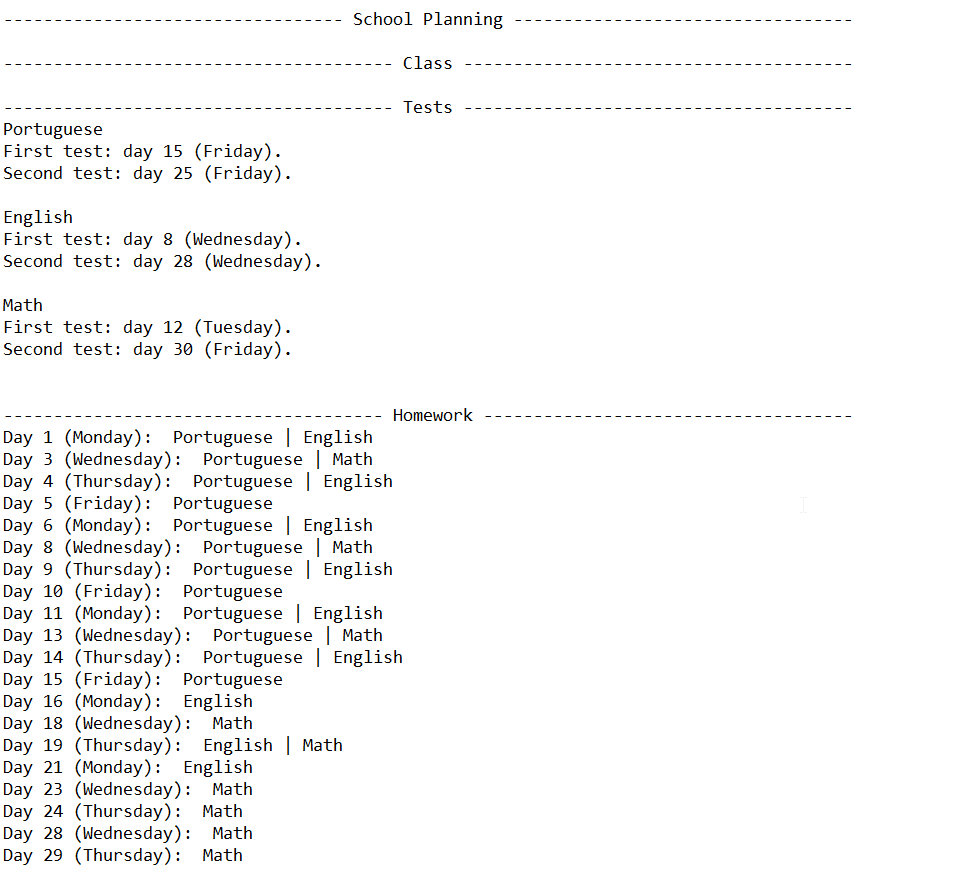
\includegraphics[scale=0.4]{images/results.png}}}

Na secção de testes, são apresentados o nome da disciplina e a data dos testes. \par
Na secção dos TPCs, são mostrados, no dia em que há TPCs, as datas em que os mesmos devem ser marcados, e para quais disciplinas.\par
O processamento da informação para \textit{output} começa no predicado \textit{display(+Classes, +Days)}, que, por sua vez, invoca o predicado \textit{displayClasses(+Classes, +Days)}, responsável por apresentar a informação de cada turma.\par
Para mostrar a informação relativamente a cada turma, é utilizado o predicado \textit{displayClass(+Class, +Days)}, e tem como função apresentar as informações relativamente às datas dos testes e dos TPCs.\newline Para mostrar os testes, é utilizado o predicado \textit{displayTests(+Class)}, que percorre todas as disciplinas de uma turma, apresentando as datas dos testes.\newline 
Para mostrar as datas dos TPCs, o predicado \textit{displayTPCs(+Class, +Day, +Days)}, percorre todos os dias, e verifica, para cada dia, quais as disciplinas que devem ter TPC, retornando uma lista com essa informação. Essa lista é depois percorrida, para formatar o \textit{output} que deverá ser mostrado ao utilizador. Desta forma, é possível mostrar somente os dias em que há TPCs marcados (ignorando as datas sem nenhum compromisso).

\section{Resultados}
Nesta secção serão mostrados os resultados da execução do programa. As variáveis a considerar são: o número de disciplinas, o número de turmas, e o número de dias.\par
No primeiro gráfico são visíveis os resultados para 3 disciplinas, variando o número de dias (entre 30 e 365) e o número de turmas (entre duas e seis):

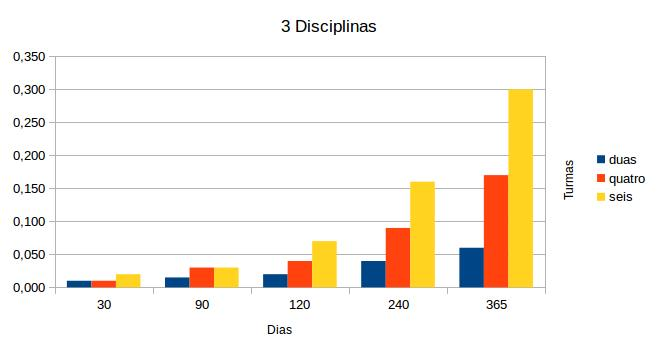
\includegraphics[scale=0.85]{images/chart1.jpg}

Os resultados mostram-se bons, sendo o tempo máximo de execução obtido \textit{0.3 segundos}.\par
\newpage
Seguidamente, o programa foi corrido num cenário de 4 disciplinas:

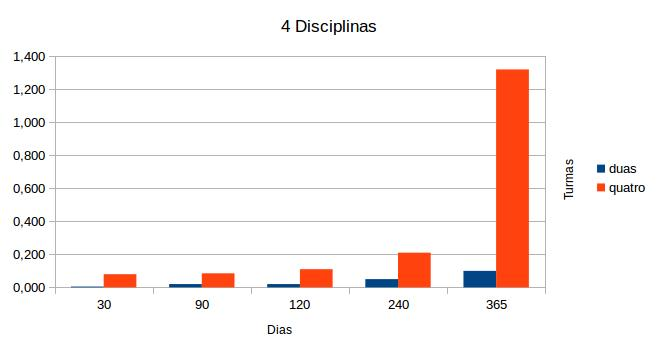
\includegraphics[scale=0.85]{images/chart2.jpg}

Note-se que não são mostrados os valores para seis turmas, pois o programa não conseguiu encontrar uma solução dentro do tempo estabelecido de 1 minuto e 30 segundos.\newline 
Os tempos de execução continuam a ser rápidos, excetuando para 4 turmas e 365 dias - que correu em \textit{1.32 segundos}, mostrando-se irregular, comparativamente aos outros resultados.

\newpage
Finalmente, as seguintes amostras foram obtidas com 6 disciplinas:

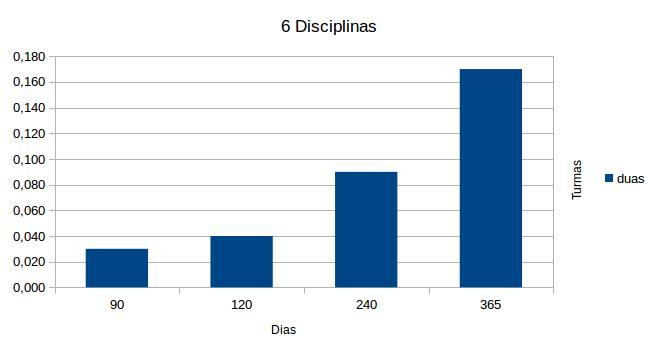
\includegraphics[scale=0.85]{images/chart3.jpg}

Os resultados não são mostrados para 4 e 6 turmas, pois, tal como aconteceu para 4 disciplinas, a solução ideal não foi encontrada no tempo estabelecido.\par

É importante referir que os tempos de execução dependem em grande escala dos \textit{inputs} dados ao programa. Os valores apresentados podem variar bastante, tendo em conta os horários das turmas.

\section{Instruções de Utilização}

Para utilizar o software desenvolvido deve ser chamado o predicado  \textit{run(+Days, +MaxTpcNumber, +NoTpcDay, +Ratio, +Schedules, -Classes)} definido no ficheiro \textit{AnoEscolar.pl}. Este predicado tem como argumentos:
	\begin{itemize}
			\item \textbf{Days} - Número de dias do periodo;
			\item \textbf{MaxTpcNumber} - Número máximo de trabalhos de casa por dia;
			\item \textbf{NoTpcDay} - Dia da semana no qual nunca existe trabalho de casa (de 1 a 5 correspondendo aos dias uteis da semana por ordem crescente);
			\item \textbf{Ratio} - Rácio de trabalhos de casa por periodo, por exemplo 2- até metade das aulas de cada disciplina podem ter trabalho de casa, 3 - até um terço das aulas de cada disciplina podem ter trabalhos de casa ;
			\item \textbf{Schedules} - hórarios de todas as turmas, consiste numa lista em que cada elemento representa um horario de uma turma, esta lista tem 5 elementos que são novamente listas com os id's das disciplinas a que tem aulas naquele dia (ex:  \textit{[ [[1,2], [2,3], [3,1], [1,2,3], [1]],  [[1,3], [2,1], [3], [2], [1,2]] ]} esta lista representa duas turmas cada uma com 3 disciplinas com id's 1 ,2 e 3); 
			\item \textbf{Classes} - Lista com todas as turmas no formato já definido anteriormente.
	\end{itemize}
Existem alguns exemplos da utilização deste predicado no ficheiro \textit{Tests.pl}, de referir ainda, que tambem pode ser utilizado o predicado  \textit{solve(+Days, +MaxTpcNumber, +NoTpcDay, +Ratio, +Schedules, -Classes)}, exatamente com os mesmos argumentos.
A vantagem de utilizar o predicado  \textit{run} é o facto de este tambem imprimir o tempo de execução do programa quando termina.




\section{Conclusões e Trabalho Futuro}
A construção deste projeto permitiu aprofundar os conhecimentos em \textit{Programação em Lógica com Restrições}, assim como pensar de forma lógica (e não funcional). Foi possível, também, conhecer o poder do \textbf{Prolog} e, em específico, do predicado \textit{labeling}, verificando como tornam possível a resolução de problemas complexos em poucas linhas de código.\par
Tendo em conta os resultados obtidos, é possível afirmar que, de uma forma geral, o programa tem tempos de execução rápidos. É, no entanto, importante notar que o aumento do número de disciplinas/turmas provoca uma diminuição na rapidez do programa mais acentuada, relativamente ao aumento do número de dias - estes últimos, apesar de dilatarem o tempo de execução, nunca foram a causa do programa não conseguir executar no tempo estabelecido.\newline
Assim sendo, pode-se afirmar que o número de dias não se trata do \textit{bottleneck} do programa, podendo este estar no número de disciplinas ou o número de turmas.\par
A principal vantagem do programa, de uma forma geral, passa pela eficiência e baixo tempo de execução. Além disso, é totalmente flexível quanto ao número de disciplinas (que devem estar na base de dados), número de turmas e número de dias, e também quanto aos horários, o número máximo de TPCs por dia, percentagem de TPCs por período e ao dia que não deve haver TPCs.\newline
No entanto, a flexibilidade nestes \textit{inputs} torna o programa pouco previsível, podendo, por vezes, haver discrepâncias nos tempos de execução. Além disso, apesar de não ter sido pedido, a aplicação poderia ser ainda mais flexibilizada - podendo receber, por exemplo, o número de testes por período.\par
A melhoria do projeto passaria, então, por flexibilizar ainda mais os \textit{inputs}, assim como identificar e melhorar a eficiência do \textit{bottleneck} da aplicação. 



%
% ---- Bibliography ----
%
\begin{thebibliography}{5}
%
\bibitem {url} 
SWI-Prolog,
\url{http://www.swi-prolog.org}
\bibitem {url} 
SICStus-Prolog,
\url{https://sicstus.sics.se}


\end{thebibliography}
\clearpage

\section*{Anexo}
\subsection*{Código fonte}
O código fonte encontra-se no diretório \textit{\textbf{code}}.

\end{document}
